%%%%%%%%%%%%%%%%%%%%%%%%%%%%%%%%%%%%%%%%%
% Beamer Presentation
% LaTeX Template
% Version 1.0 (10/11/12)
%
% This template has been downloaded from:
% http://www.LaTeXTemplates.com
%
% License:
% CC BY-NC-SA 3.0 (http://creativecommons.org/licenses/by-nc-sa/3.0/)
%
%%%%%%%%%%%%%%%%%%%%%%%%%%%%%%%%%%%%%%%%%

%----------------------------------------------------------------------------------------
%	PACKAGES AND THEMES
%----------------------------------------------------------------------------------------

\documentclass{beamer}

\mode<presentation> {

% The Beamer class comes with a number of default slide themes
% which change the colors and layouts of slides. Below this is a list
% of all the themes, uncomment each in turn to see what they look like.

\usetheme{default}
%\usetheme{AnnArbor}
%\usetheme{Antibes}
%\usetheme{Bergen}
%\usetheme{Berkeley}
%\usetheme{Berlin}
%\usetheme{Boadilla}
%\usetheme{CambridgeUS}
%\usetheme{Copenhagen}
%\usetheme{Darmstadt}
%\usetheme{Dresden}
%\usetheme{Frankfurt}
%\usetheme{Goettingen}
%\usetheme{Hannover}
%\usetheme{Ilmenau}
%\usetheme{JuanLesPins}
%\usetheme{Luebeck}
%\usetheme{Madrid}
%\usetheme{Malmoe}
%\usetheme{Marburg}
%\usetheme{Montpellier}
%\usetheme{PaloAlto}
%\usetheme{Pittsburgh}
%\usetheme{Rochester}
%\usetheme{Singapore}
%\usetheme{Szeged}
%\usetheme{Warsaw}

% As well as themes, the Beamer class has a number of color themes
% for any slide theme. Uncomment each of these in turn to see how it
% changes the colors of your current slide theme.

%\usecolortheme{albatross}
%\usecolortheme{beaver}
%\usecolortheme{beetle}
%\usecolortheme{crane}
%\usecolortheme{dolphin}
%\usecolortheme{dove}
%\usecolortheme{fly}
%\usecolortheme{lily}
%\usecolortheme{orchid}
%\usecolortheme{rose}
%\usecolortheme{seagull}
%\usecolortheme{seahorse}
%\usecolortheme{whale}
%\usecolortheme{wolverine}

%\setbeamertemplate{footline} % To remove the footer line in all slides uncomment this line
%\setbeamertemplate{footline}[page number] % To replace the footer line in all slides with a simple slide count uncomment this line

%\setbeamertemplate{navigation symbols}{} % To remove the navigation symbols from the bottom of all slides uncomment this line
}

\usepackage{graphicx} % Allows including images
\usepackage{booktabs} % Allows the use of \toprule, \midrule and \bottomrule in tables
\usepackage{url}
\usepackage[T1]{fontenc}
\usepackage[utf8]{inputenc}
\usepackage{listings}
\usepackage{adjustbox}
\lstset{language=C++,
  basicstyle=\footnotesize\ttfamily,
  keywordstyle=\footnotesize\color{blue}\ttfamily,
}
%----------------------------------------------------------------------------------------
%	TITLE PAGE
%----------------------------------------------------------------------------------------

\title[Forward Kinematics]{Programming Exercises 3.1 and 3.2} % The short title appears at the bottom of every slide, the full title is only on the title page

\author{Kasper Høj Lorenzen} % Your name
\institute[SDU Robotics] % Your institution as it will appear on the bottom of every slide, may be shorthand to save space
{
University of Southern Denmark \\ % Your institution for the title page
\medskip
\textit{kalor@mmmi.sdu.dk} % Your email address
}
\date{September 14, 2022} % Date, can be changed to a custom date

\begin{document}

\begin{frame}
\titlepage % Print the title page as the first slide
\end{frame}

\begin{frame}
\frametitle{Overview} % Table of contents slide, comment this block out to remove it
\tableofcontents % Throughout your presentation, if you choose to use \section{} and \subsection{} commands, these will automatically be printed on this slide as an overview of your presentation
\end{frame}

%----------------------------------------------------------------------------------------
%	PRESENTATION SLIDES
%----------------------------------------------------------------------------------------

%------------------------------------------------
\section{Programming Exercise 1.2} % Sections can be created in order to organize your presentation into discrete blocks, all sections and subsections are automatically printed in the table of contents as an overview of the talk
%------------------------------------------------

\begin{frame}
  \frametitle{Programming Exercise 1.2}
  \begin{columns}
    \begin{column}{0.5\textwidth}
      \begin{center}
        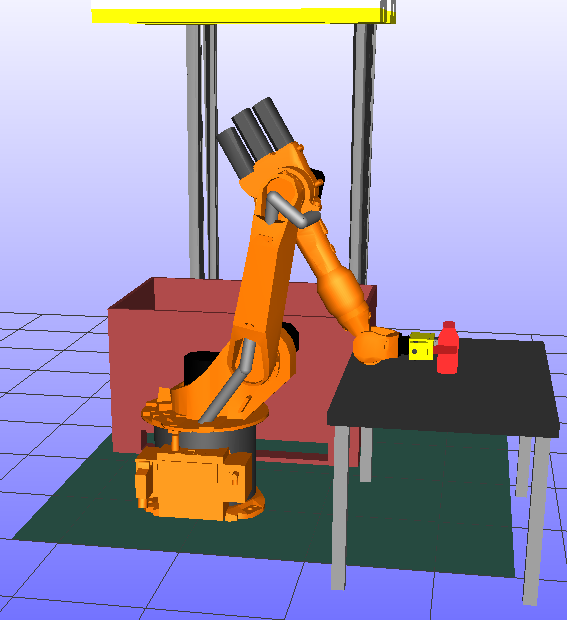
\includegraphics[height=0.5\textheight]{./graphics/ex22sol1}
        \begin{itemize}
        \item \resizebox{\linewidth}{!}{\texttt{q=\{1.7712, -0.0548906, -2.41234, 2.88718, 0.912336, -1.413\}}} % Q[6]{1.7712, -0.0548906, -2.41234, 2.88718, 0.912336, -1.413}
        \item \resizebox{\linewidth}{!}{\texttt{q=\{1.76941, -0.0565661, -2.41395, 2.88328, 0.910975, 4.71239\}}} % Q[6]{1.76941, -0.0565661, -2.41395, 2.88328, 0.910975, 4.71239}
        \end{itemize}
      \end{center}
    \end{column}
    \begin{column}{0.5\textwidth}
      \begin{center}
        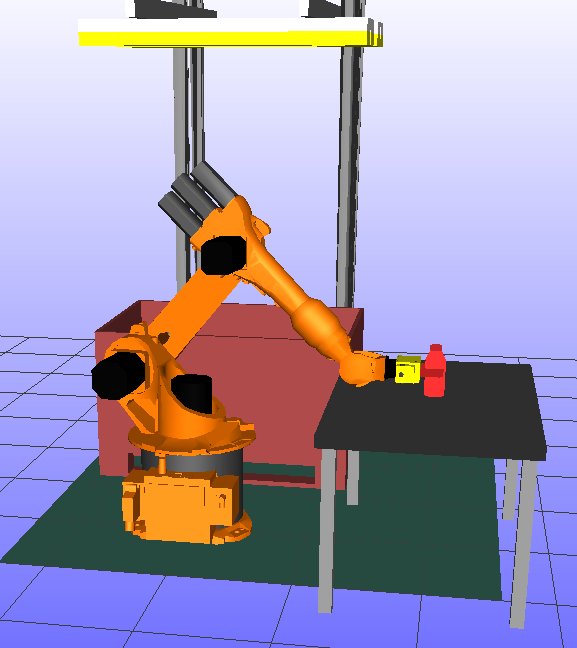
\includegraphics[height=0.5\textheight]{./graphics/ex22sol2}
      \begin{itemize}
      \item \resizebox{\linewidth}{!}{\texttt{q=\{-1.42764, 0.66059, 1.56711, 6.05139, 0.670049, -1.38785\}}}
      \item \resizebox{\linewidth}{!}{\texttt{q=\{-1.42899, 0.662597, 1.56841, 6.05942, 0.672475, 4.88856\}}}
      \end{itemize}
      \end{center}
      
    \end{column}
  \end{columns}
\begin{itemize}
\item Additional solutions if joint limits are relaxed
\end{itemize}
\end{frame}

%------------------------------------------------


%------------------------------------------------
\section{Programming Exercise 2} % Sections can be created in order to organize your presentation into discrete blocks, all sections and subsections are automatically printed in the table of contents as an overview of the talk
%------------------------------------------------

\begin{frame}
  \frametitle{Programming Exercise 2}
  \begin{columns}
    \begin{column}{0.6\textwidth}
      \begin{itemize}
      \item Solution is on itslearning
      \end{itemize}
    \end{column}
    \begin{column}{0.4\textwidth}
      \begin{centering}
        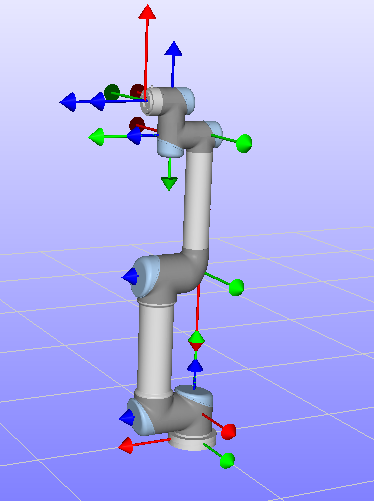
\includegraphics[width=0.7\textwidth]{./graphics/ex33_sol}
      \end{centering}
    \end{column}
  \end{columns}
\end{frame}

%------------------------------------------------

\section{RobWork math and workcells}

% ------------------------------------------------

\begin{frame}
  \frametitle{RobWork Math}
  \begin{itemize}
  \item RobWork includes types for all the transformations used in this course
  \item Take a look at the HelloRobwork program to see usage of the various transformations
  \item There is also a \texttt{Rotation3D} class
  \item Take a look at \url{http://www.robwork.dk/apidoc/cpp/doxygen/namespacerw_1_1math.html} and the Python API to see what other types there are
  \end{itemize}
\end{frame}

% ------------------------------------------------

\begin{frame}[fragile]
  \frametitle{Loading a workcell with RobWork}
  \begin{itemize}
  \item Workcells can be loaded into C++ and Python using RobWork
  \item See the pages for \texttt{WorkCell} and \texttt{Device} on \url{www.robwork.dk}
  \end{itemize}
  
  \begin{adjustbox}{width=\textwidth,keepaspectratio}
    \begin{lstlisting}
      const string workcell_path = "/path/to/workcell/Scene.wc.xml";
      const string device_name = "device_name";
      WorkCell::Ptr wc = WorkCellLoader::Factory::load(workcell_path);
      Device::Ptr device = wc->findDevice(device_name);
    \end{lstlisting}
  \end{adjustbox}
  
\end{frame}


\section{Programming Exercises 3.2}

% ------------------------------------------------

\begin{frame}
  \frametitle{Programming Exercise 3.2}
  \begin{itemize}
  \item Program a function to calculate the forward kinemactics
  \item \texttt{Transform3D} can be used to represent the transformations $\mathbf{T}$
  \item \texttt{Q} can be used for the state vector $\mathbf{q}$
    \item Compare your solution to the workcell UR-6-85-5-A WorkCell
  \end{itemize}
\end{frame}


% ------------------------------------------------

\section{Programming Exercises 3.1}

% ------------------------------------------------


\begin{frame}
  \frametitle{Programming Exercise 3.1}
  \begin{itemize}
  \item Program a function to calculate the Jacobian
  \item The built-in type \texttt{Jacobian} can be used to represent the Jacobian $\mathbf{J(q)}$
  \item Give the function a vector of Transforms, solve for the A and B part and merge it
    %\item Compare your solution to the example in section 4.3.1
  \end{itemize}
\end{frame}

% \begin{frame}
%\frametitle{References}
%\footnotesize{
%\begin{thebibliography}{99} % Beamer does not support BibTeX so references must be inserted manually as below
%\bibitem[Ellekilde, Jorgensen, 2010]{robwork} L. P. Ellekilde and J. A. Jorgensen (2010)
%\newblock RobWork: A Flexible Toolbox for Robotics Research and Education
%\newblock \emph{ISR 2010 (41st International Symposium on Robotics) and ROBOTIK 2010 (6th German Conference on Robotics)}, 1 -- 7.
%\end{thebibliography}
%}
%\end{frame}

%----------------------------------------------------------------------------------------

\end{document} 
